\documentclass[11 pt]{article} 
\usepackage[left=2cm, top=2cm, right=2cm, bottom=2.5cm, footskip=.5cm]{geometry}
\usepackage{graphicx}
\usepackage{subcaption} 
\usepackage{subfig}
\usepackage{amsmath}
\usepackage{url}
\usepackage{booktabs}
\usepackage{units}
\usepackage{enumitem}
\usepackage{listings}
\usepackage{float}
 \usepackage{booktabs}
 
\author{Natalia Zuniga-Garcia}
\title{Exercises 1 Preliminaries}
\date{\today}

\begin{document}
\maketitle

\section{Linear Regression}\label{sec:linr}
Consider the simple linear regression model
$$
y = X \beta + e \, ,
$$
where $y = (y_1, \ldots, y_N)$ is an $N$-vector of responses, $X$ is an $N \times P$ matrix of features whose $i$th row is $x_i$, and $e$ is a vector of model residuals.  The goal is to estimate $\beta$, the unknown $P$-vector of regression coefficients.  

Let's say you trust the precision of some observations more than others, and therefore decide to estimate $\beta$ by the principle of weighted least squares (WLS):
$$
\hat{\beta} = \arg \min_{\beta \in \mathcal{R}^P} \sum_{i=1}^N \frac{w_i}{2}(y_i - x_i^T \beta)^2 \, ,
$$
where $w_i$ is the weight for observation $i$.  (Higher weight means more influence on the answer; the factor of 1/2 is just for convenience, as you'll see later.)

\begin{enumerate}[label=(\Alph*)]

\item Rewrite the WLS objective function\footnote{That is, the thing to be minimized.} above in terms of vectors and matrices, and show that $\hat \beta$ is the solution to the following linear system of $P$ equations in $P$ unknowns:
$$(X^T W X) \hat \beta = X^T W y $$ where $W$ is the diagonal matrix of weights.

\vspace{2mm}
\textbf{Solution}

In matrix notation, let  $W$ be a diagonal matrix containing the scaled  $w_i$  along the diagonal and zeros elsewhere, and let $y$ and $X$ be the matrices associated with $y_i $ and $x_i $, respectively Then, we can write the WLS estimator as follow,
$$\hat{\beta} = \arg \min_{\beta \in \mathcal{R}^P} \sum_{i=1}^N \frac{w_i}{2}(y_i - x_i^T \beta)^2 
=arg \min_{\beta \in \mathcal{R}^P}\Bigg[ \frac{1}{2}\sum_{i=1}^N y_iw_iy_i -\sum_{i=1}^N x_i^T\beta w_iy_i + \frac{1}{2}\sum_{i=1}^N x_i^T\beta w_ix_i^T\beta\Bigg]$$
$$\hat{\beta} =arg \min_{\beta \in \mathcal{R}^P}\bigg[\frac{1}{2}y^TWy-X^T\beta^T Wy+\frac{1}{2}X^T\beta^T WX\beta\bigg]=arg \min_{\beta \in \mathcal{R}^P}\bigg[\frac{1}{2}(y-X\beta)^TW(y-X\beta)\bigg]$$

Now we try to minimize the WLS objective function by calculating its gradient and equalizing it to zero as follow,
$$\nabla(\hat{\beta})=0$$
$$\nabla(\hat{\beta})=0-X^TWy+\frac{2}{2}X^TWX\hat \beta=0 \Rightarrow (X^T W X) \hat \beta = X^T W y $$

\newpage
\item One way to calculate $\hat{\beta}$ is to: (1) recognize that, trivially, the solution to the above linear system must satisfy $\hat \beta = (X^T W X)^{-1} X^T W y$; and (2) to calculate this directly, i.e.~by inverting $X^T W X$.  Let's call this the ``inversion method'' for calculating the WLS solution.

Numerically speaking, is the inversion method the fastest and most stable way to actually solve the above linear system?  Do some independent sleuthing on this question.  Summarize what you find, and provide pseudo-code for at least one alternate method based on matrix factorizations---call it ``your method'' for short.  (Note: our linear system is not a special flower; whatever you discover about general linear systems should apply here.)

\vspace{2mm}
\textbf{Solution}

It is always recommended to avoid inverting matrices due to numerical stability. The ``inversion method" is only possible if the matrix $X^T W X$ is ``well behaved", i.e. it is full rank corresponding to linearly independent columns in X \cite{nielsen2007}. The system of normal equations should not be solved by inverting $X^T W X$ for reasons of numerical stability especially in situations with nearly linear dependencies between the columns of X (causing slight alterations to the observed values in X to lead to substantial changes in the estimated $\hat \beta$, this problem is known as multicollinearity) \cite{nielsen2007}. 

Alternate methods for solving the system of normal equations are: Singular Value Decomposition (SVD), QR Decomposition or Cholesky Decomposition. The method I choose as "my method" is Cholesky Decomposition. The pseudo-code is presented as follow,
\begin{itemize}
	\item First, we factorize $X^T W X$ using the Cholesky Decomposition as:
	$$X^T W X = C^TC$$
	Where, C is upper triangular.
	\item Now we have:
		$$X^TWX \hat \beta = X^T W y$$
		$$C^TC \hat \beta = X^T W y$$
	This system of equations can be solved by two times back-substitution:
		$$C^T(C \hat \beta) = X^T W y$$
		$$C \hat \beta = C^{-T} X^T W y$$
	Let's call $z=C \hat \beta$ and solve for $z$ by estimating: 
	$$z=C^{-T} X^T W y$$
	\item And then, we can solve for $\hat \beta$ as follow:
			$$\hat \beta = C^{-1} z$$
\end{itemize}
Solving a linear system equires a time complexity of $O(n^3)$. Although the Cholesky Decomposition still have  $O(n^3)$, the back-substitution steps require  $O(n^2)$ \cite{krishna2013}, which makes this method faster than the ``inversion method".

\newpage
\item Code up functions that implement both the inversion method and your method for an arbitrary $X$, $y$, and weights $W$.  Obviously you shouldn't write your own linear algebra routines for doing things like multiplying or decomposing matrices, but don't use a direct model-fitting function like R's ``lm'' either.   Your actual code should look a lot like the pseudo-code you wrote for the previous part.  Note: be attentive to how you multiply a matrix by a diagonal matrix, or you'll waste a lot of time multiplying stuff by zero.

\vspace{2mm}
\textbf{Solution}

The functions\footnote{The solution is presented in the file $P1C1Functions.R$} for the ``inversion method"  and ``my method" (corresponding to the Cholesky Decomposition) are: 
\begin{lstlisting}[language=R]

# Implementation of functions to calculate the 
# Weighted Least Squares (WLS) solution

# Function 1. Inversion Method
inv.method <- function(X,y,W){
# X is an N x P matrix
# y is the N-vector of response
# W is the N x N diagonal matrix of weights
# The output is b.hat, the unknown P-vector of regression coefficients
# Let's solve b.hat=A^(-1)B where A=X^TWX and B=X^TWy
A.inv = solve(crossprod(X,diag(W)*X))
B = crossprod(X,diag(W)*y)
return(crossprod(A.inv, B)) # Solving for b.hat
}

# Function 2. My Method (using Cholesky Decomposition)
my.method <- function(X,y,W){
# X is an N x P matrix
# y is the N-vector of response
# W is the N x N diagonal matrix of weights
# The output is b.hat, the unknown P-vector of regression coefficients 
# Let's solve A(b.hat)=B where A=X^TWX=C^TC and B=X^TWy
C = chol(crossprod(X,diag(W)*X)) 
# Using the Cholesky Decomposition C^TC
# for A=X^TWX where C is upper tringle
B = crossprod(X,diag(W)*y)
z = forwardsolve (t(C), B) # Solving for z in C^Tz=X^TWy 
# Where C^T is lower tringle 
b.hat = backsolve(C,z) # Solving for b.hat in C(b.hat)=z
# Where C is upper triangle 
return(b.hat)
}
\end{lstlisting}



\newpage
Now simulate some silly data from the linear model for a range of values of $N$ and $P$.  (Feel free to assume that the weights $w_i$ are all 1.)  It doesn't matter how you do this---e.g.~everything can be Gaussian if you want.  (We're not concerned with statistical principles yet, just with algorithms, and using least squares is a pretty terrible idea for enormous linear models, anyway.)  Just make sure that you explore values of $P$ up into the thousands, and that $N > P$.  Benchmark the performance of the inversion solver and your solver across a range of scenarios.  (In R, a simple library for this purpose is microbenchmark.)

\vspace{2mm}
\textbf{Solution}

The results\footnote{The solution is presented in the file $P1C2Simulation.R$.} are shown Figure \ref{fig:Fig1}. The simulated data consisted of a range of P values with a fixed N of 2000, and a range of N values with a fixed P of 100. The values of N correspond to the number of linear equations we are going to solve, while the values of P correspond to the number of unknowns we have. The methods evaluated are the  ``inversion method" and ``my method" which uses the Cholesky Decomposition.

We can observe that when increasing the P values, the method that uses the Cholesky Decomposition (``my method") presents significant lower computation time. The difference is notable when P is in the order of thousands. 
 
When varying the N values, the computational time of the two methods is similar. However, ``my method" presents results better in terms of computational times compared to the ``inversion method" for large values of N.

\begin{figure}[H]
	\begin{center}
	\begin{subfigure}[h]{0.45\linewidth}
		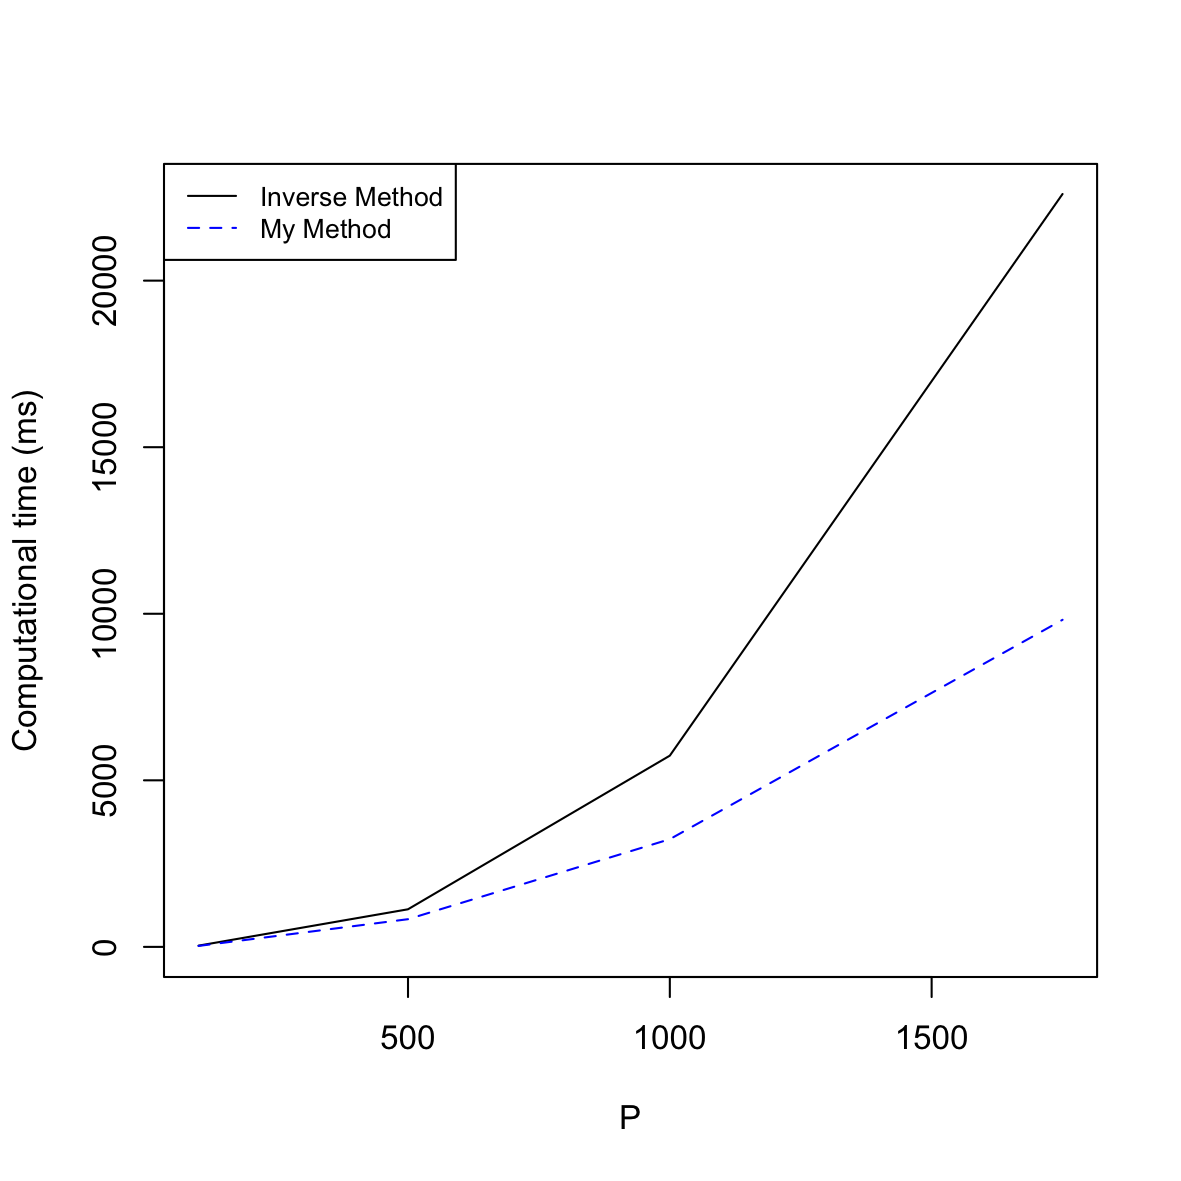
\includegraphics[width=\linewidth]{Ex01R/Fig/P1CP.png}
		\caption{N=2000, and a range of values of P}
	\end{subfigure}
	\begin{subfigure}[h]{0.45\linewidth}
		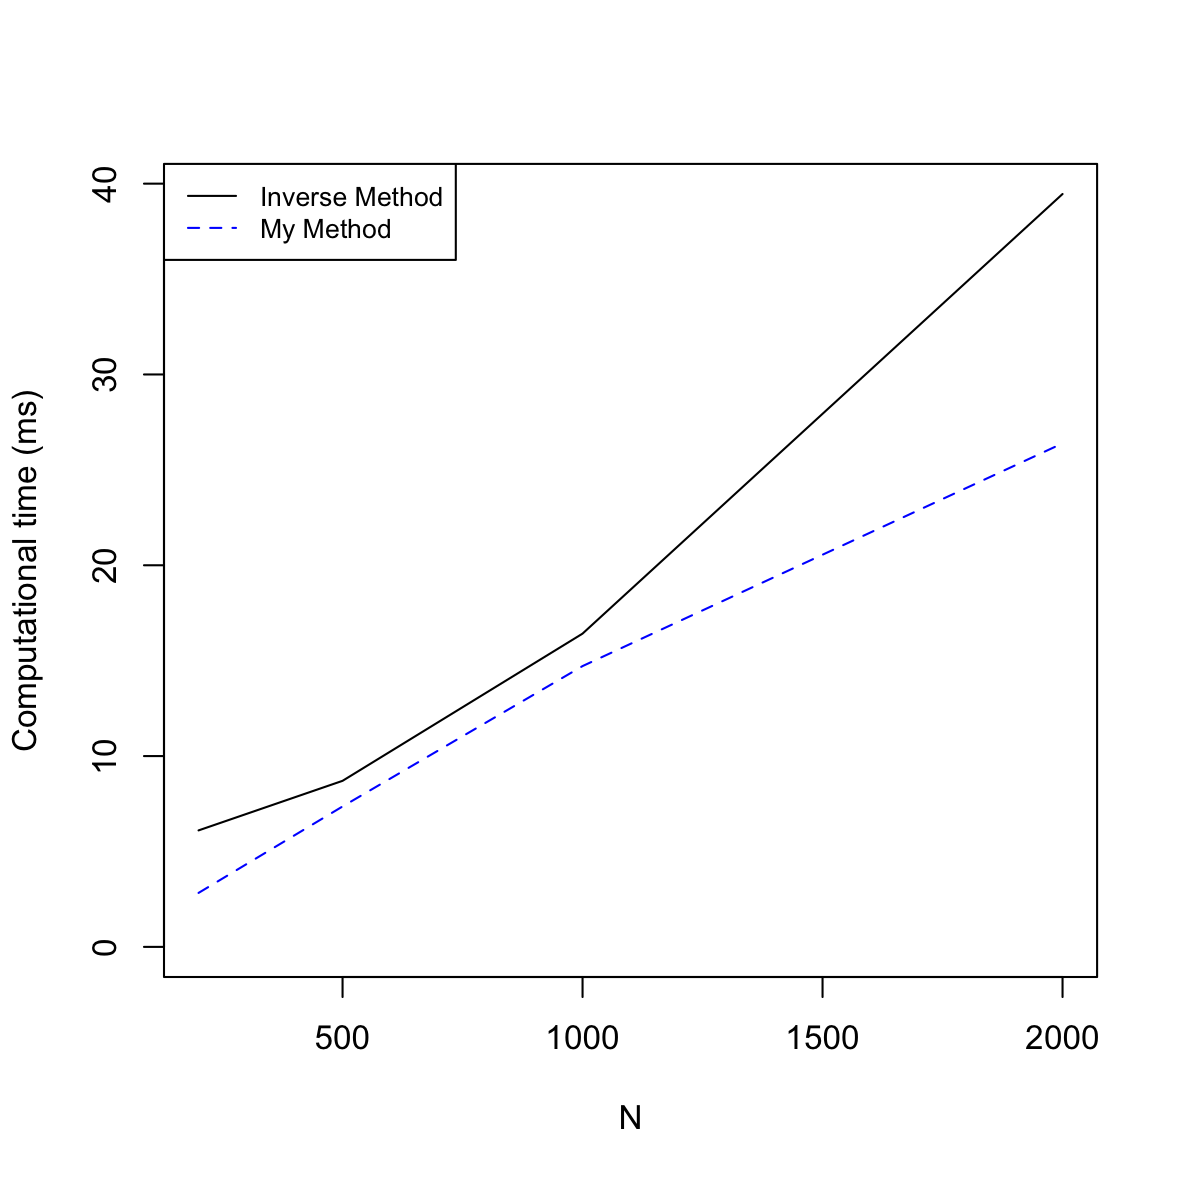
\includegraphics[width=\linewidth]{Ex01R/Fig/P1CN.png}
		\caption{P=100, and a range of values of N}
	\end{subfigure}%
	\caption{Simulation of data from linear models}
\label{fig:Fig1}
\end{center}
\end{figure}

\newpage
\item Now what happens if $X$ is a highly sparse matrix, in the sense that most entries are zero?  Ideally we'd realize some savings by not doing a whole bunch of needless multiplication by zero in our code.

It's easy to simulate an $X$ matrix that looks like this.  A quick-and-dirty way is to simulate a mask of zeros and ones (but mostly zeros), and then do pointwise multiplication with your original feature matrix.  For example:
\begin{verbatim}
N = 2000
P = 500
X = matrix(rnorm(N*P), nrow=N)
mask = matrix(rbinom(N*P,1,0.05), nrow=N)
X = mask*X
X[1:10, 1:10]  # quick visual check
\end{verbatim}

Again assume that the weights $w_i$ are all 1.  Repeat the previous benchmarking exercise with this new recipe for simulating a sparse $X$, except add another solver to the mix: one that can solve a linear system $Ax = b$ in a way that exploits the sparsity of A.  To do this, you'll need to actually represent the feature matrix $X$ in a sparse format, and then call the appropriate routines  for that format.  (Again, do some sleuthing; in R, the Matrix library has data structures and functions that can do this; SciPy will have an equivalent.)

Benchmark the inversion method, your method, and the sparse method across some different scenarios (including different sparsity levels in $X$, e.g. 5\% dense in my code above).


\vspace{2mm}
\textbf{Solution}

Literature suggests two main packages  that support sparse matrices: the $Matrix$, and the $Slam$ packages \cite{john2011}. The author presented an example of a 1000 x 1000 zero-matrix, the object sizes were:
\begin{itemize}
	\item 8000200 bytes when using $matrix$
	\item 5632 bytes when using $Matrix$ from Matrix library
	\item 1032 bytes when using $simple-triple-zero-matrix$ from the Slam Library
\end{itemize}

The function\footnote{The solution is presented in the file $P1D1Function.R$} implementation in this exercise uses $Matrix$ from Matrix library during the implementation of the  Cholesky Decomposition method. This functions is called ``my sparse method":
\newpage
\begin{lstlisting}[language=R]

# Implementation of functions to calculate the 
# Weighted Least Squares (WLS) solution in a highly sparse matrix

library(Matrix) # Library to use in sparse matrices

# Function 3. My Sparse Method (using Cholesky Decomposition)
mysparse.method <- function(X,y,W){
# X is an N x P matrix and y is the N-vector of response
# W is the N x N diagonal matrix of weights
# The output is b.hat, the unknown P-vector of regression coefficients 
# Let's solve A(b.hat)=B where A=X^TWX=C^TC and B=X^TWy
# In addition we have that X is an sparse matrix so we exploit its sparsity
X = Matrix(X, sparse=TRUE) # Sparsity
C = chol(crossprod(X,diag(W)*X)) 
# Using the Cholesky Decomposition C^TC
# for A=X^TWX where C is upper tringle
B = crossprod(X,diag(W)*y)
z = forwardsolve (t(C), B) # Solving for z in C^Tz=X^TWy 
# Where C^T is lower tringle 
b.hat = backsolve(C,z) # Solving for b.hat in C(b.hat)=z
# Where C is upper triangle 
return(b.hat)
}
\end{lstlisting}

The results\footnote{The solution is presented in the file $P1D2Simulation.R$.} are shown Figure \ref{fig:Fig2}. Similarly to the previous section, the simulated data consisted of a range of P values with a fixed N of 2000, and a range of N values with a fixed P of 100. In addition, three different sparsity ($e$) scenarios where tested: 0.05, 0.50, and 0.75. The methods evaluated are the  ``inversion method", ``my method" which uses the Cholesky Decomposition, and ``my sparse method" which also uses Cholesky Decomposition but exploits the sparsity of the matrix $X$ using the Matrix library.

We can observe that ``my sparse method" has significantly lower computational time compared to the others methods, when varying P. In addition, as the sparsity level increases, the computational time also increases, but the other methods remain constant. 
\newpage

\begin{figure}[H]
	\begin{center}
		\begin{subfigure}[h]{0.45\linewidth}
			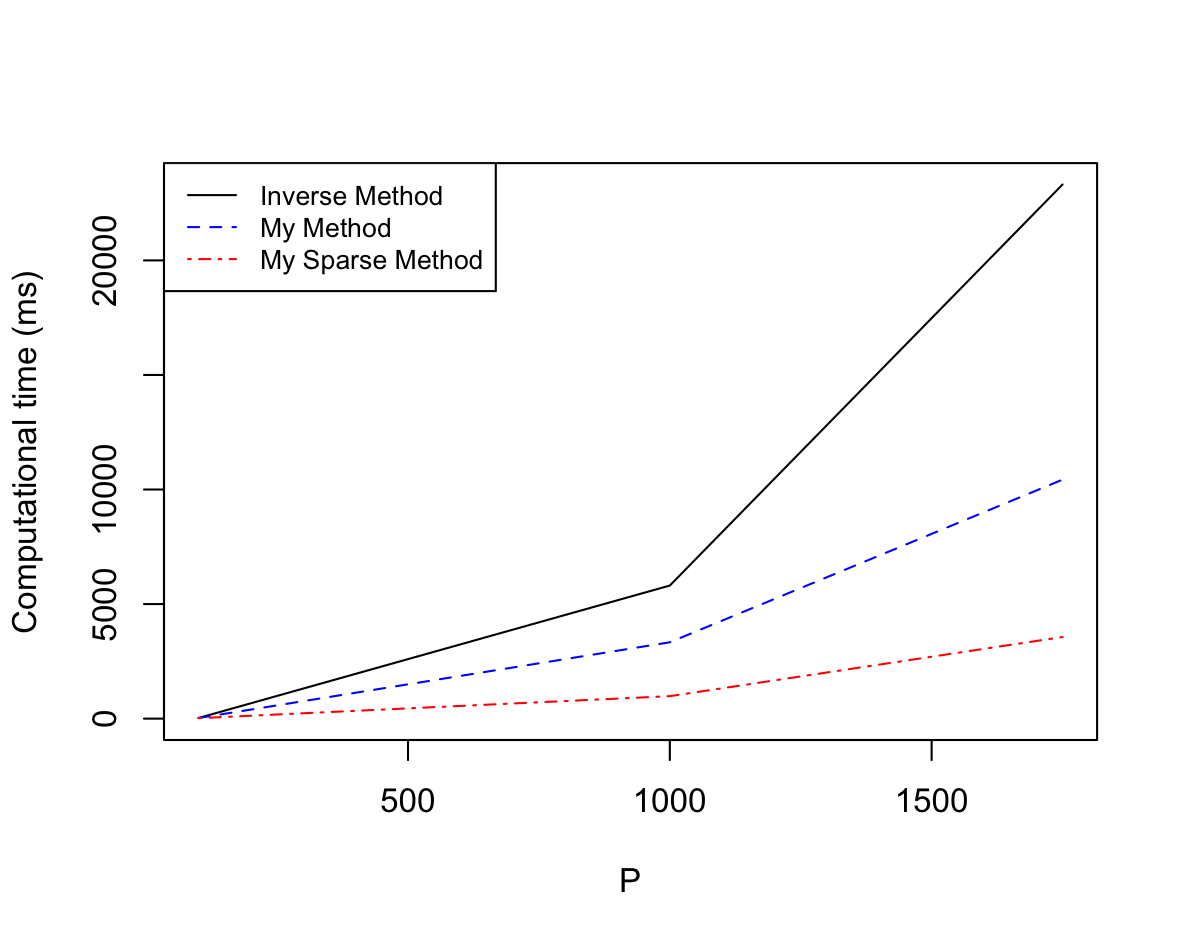
\includegraphics[width=\linewidth]{Ex01R/Fig/P1DPe005.png}
			\caption{e=0.05, N=2000, and a range of values of P}
		\end{subfigure}
		\begin{subfigure}[h]{0.45\linewidth}
			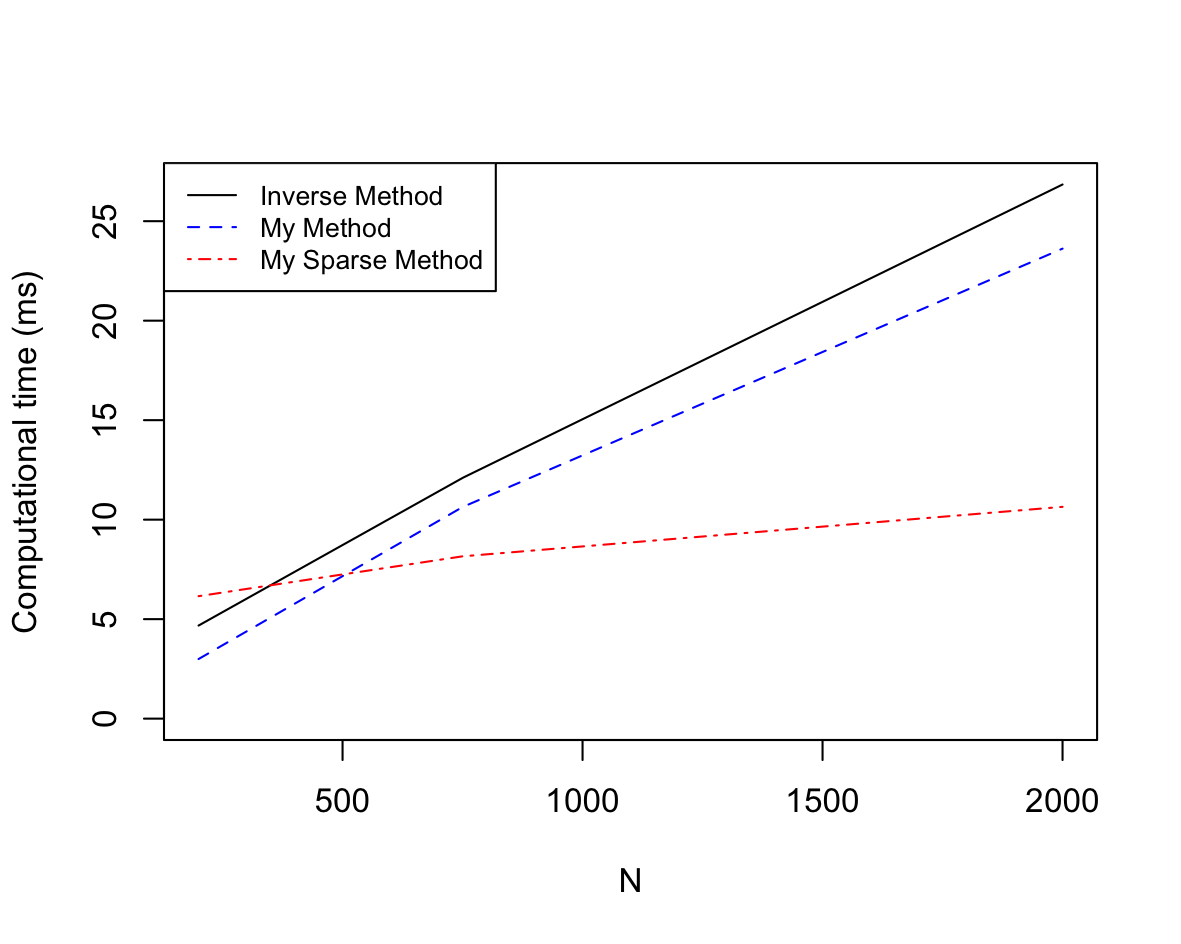
\includegraphics[width=\linewidth]{Ex01R/Fig/P1DNe005.png}
			\caption{e=0.05, P=100, and a range of values of N}
		\end{subfigure}
			\begin{subfigure}[h]{0.45\linewidth}
		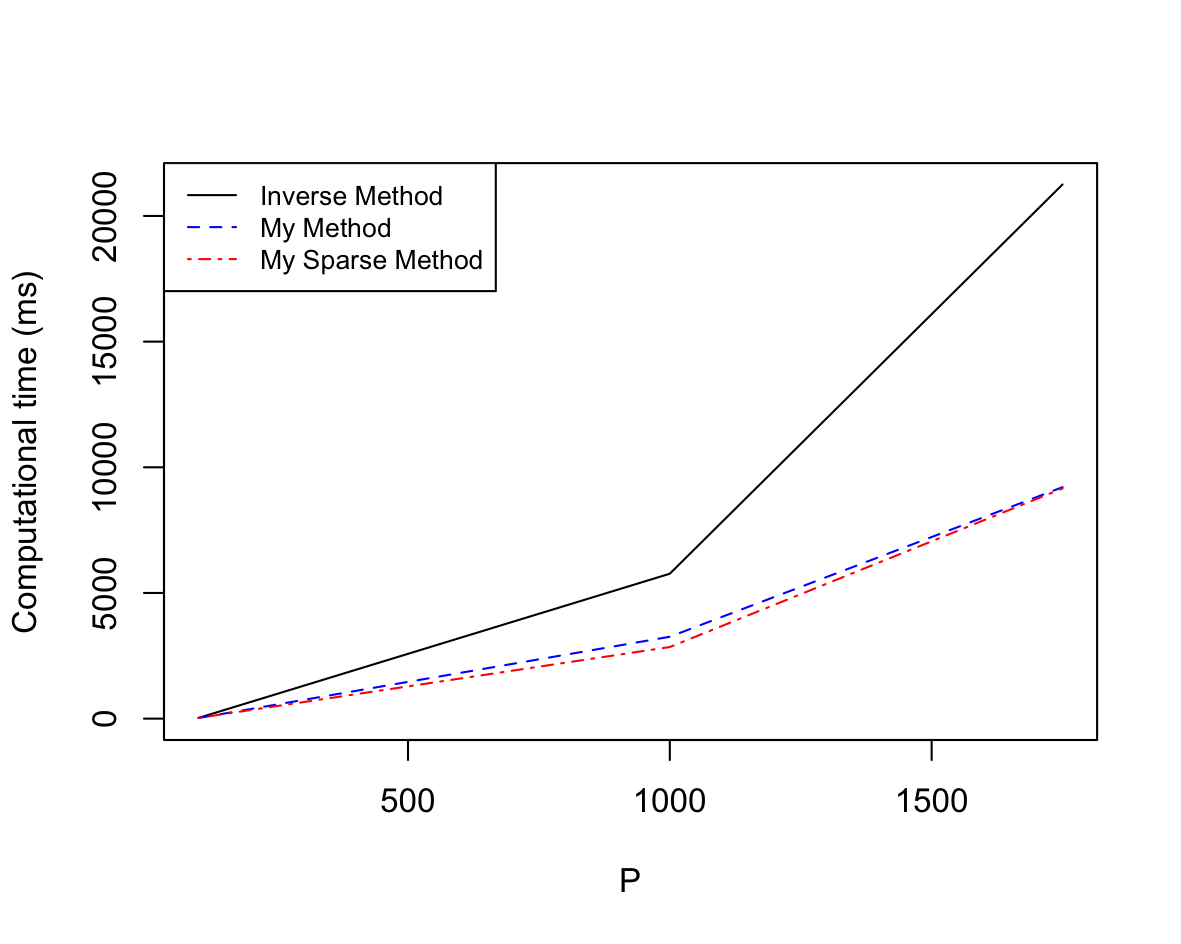
\includegraphics[width=\linewidth]{Ex01R/Fig/P1DPe05.png}
		\caption{e=0.50, N=2000, and a range of values of P}
	\end{subfigure}
		\begin{subfigure}[h]{0.45\linewidth}
	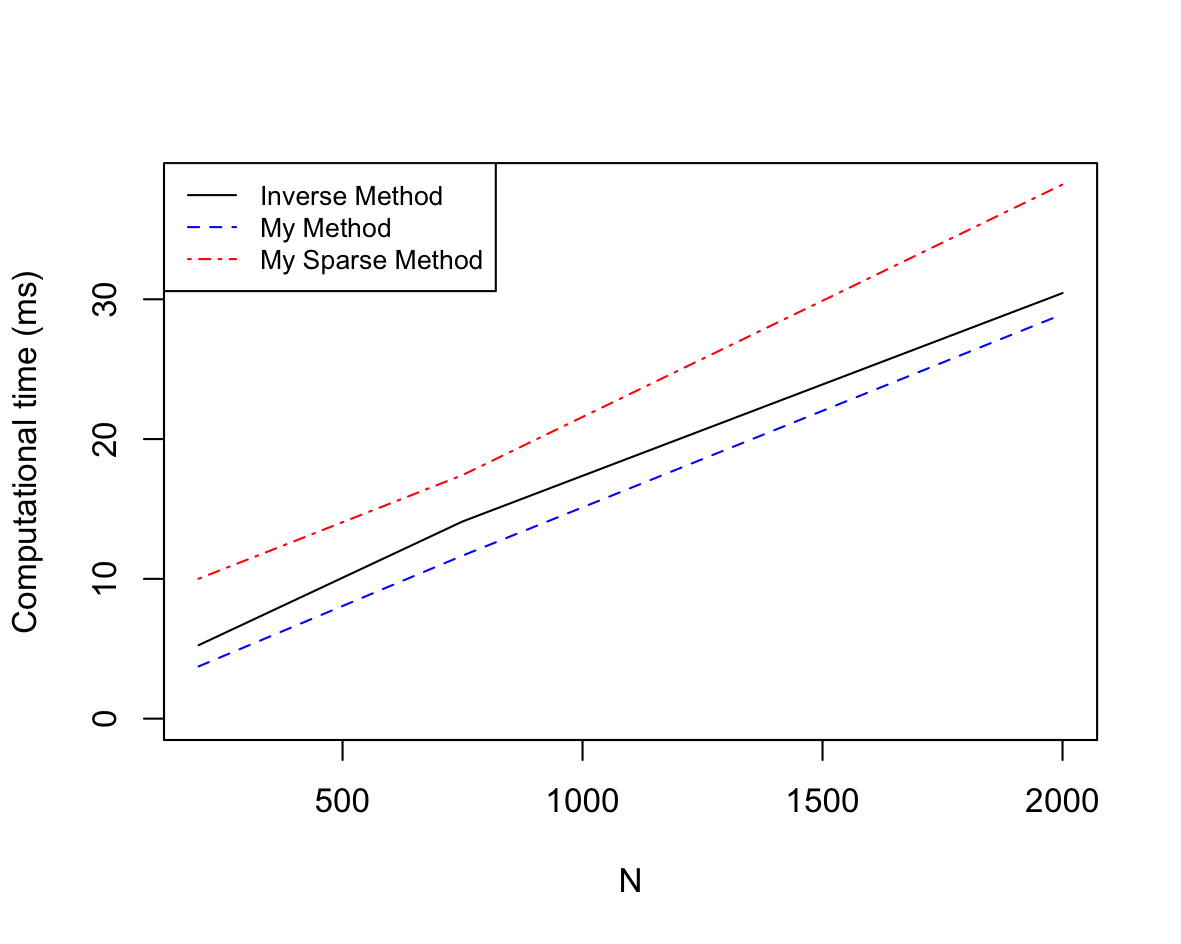
\includegraphics[width=\linewidth]{Ex01R/Fig/P1DNe05.png}
	\caption{e=0.50, P=100, and a range of values of N}
	\end{subfigure}
		\begin{subfigure}[h]{0.45\linewidth}
	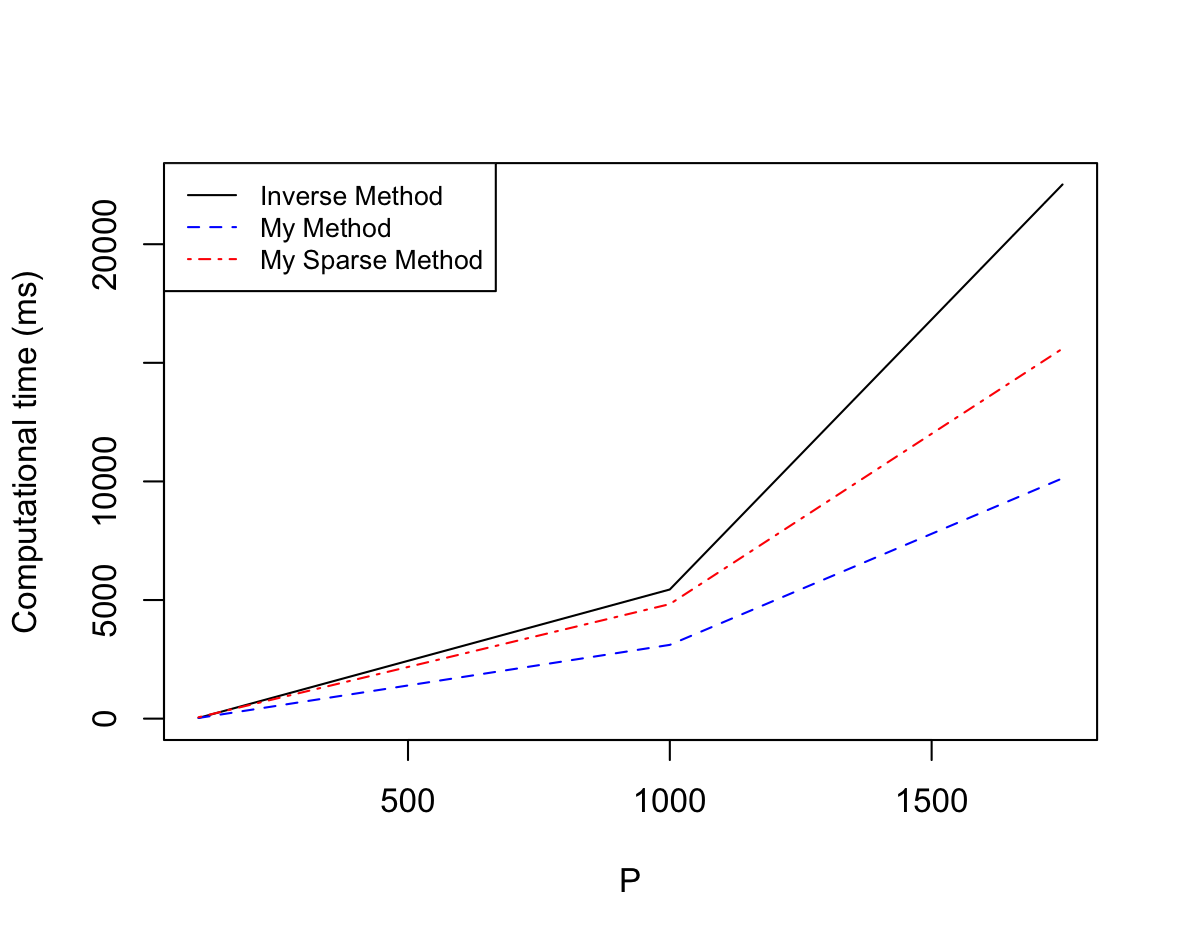
\includegraphics[width=\linewidth]{Ex01R/Fig/P1DPe075.png}
	\caption{e=0.75, N=2000, and a range of values of P}
	\end{subfigure}
		\begin{subfigure}[h]{0.45\linewidth}
	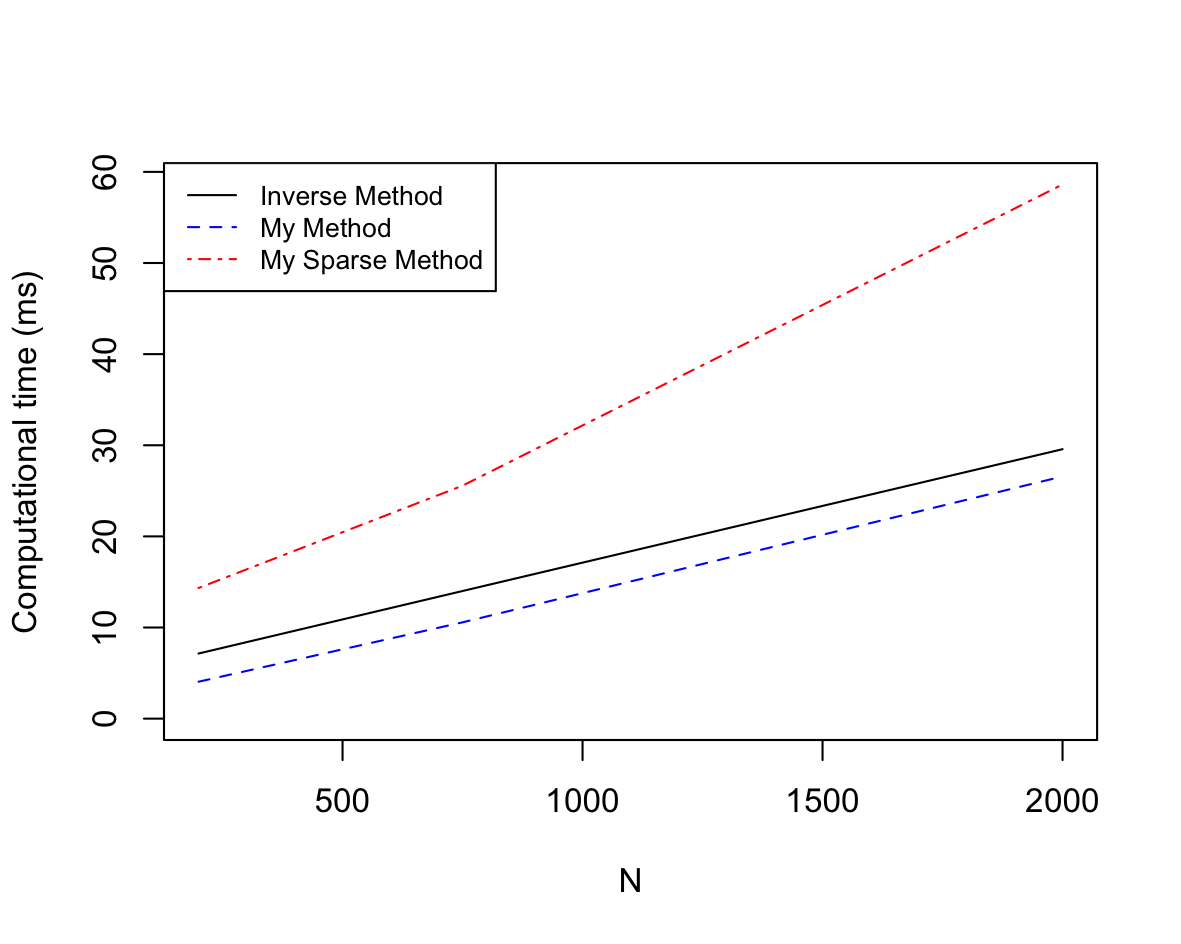
\includegraphics[width=\linewidth]{Ex01R/Fig/P1DNe075.png}
	\caption{e=0.75, P=100, and a range of values of N}
	\end{subfigure}
		\caption{Simulation of data from linear models in sparse matrices}
		\label{fig:Fig2}
	\end{center}
\end{figure}


\end{enumerate}
\newpage
\section{Generalized Linear Models}\label{sec:method}

As an archetypal case of a GLM, we'll consider the binomial logistic regression model: $y_i \sim \mbox{Binomial}(m_i, w_i)$, where $y_i$ in an integer number of ``successes,'' $m_i$ is the number of trials for the $i$th case, and the success probability $w_i$ is a regression on a feature vector $x_i$ given by the inverse logit transform:
$$
w_i = \frac{1}{1 + \exp\{-x_i^T \beta\}} \, .
$$
We want to estimate $\beta$ by the principle of maximum likelihood.  Note: for binary logistic regression, $m_i = 1$ and $y_i$ is either 0 or 1.

As an aside, if you have a favorite data set or problem that involves a different GLM---say, a Poisson regression for count data---then feel free to work with that model instead throughout this entire section.  The fact that we're working with a logistic regression isn't essential here; any GLM will do.

\begin{enumerate}[label=(\Alph*)]

\item Start by writing out the negative log likelihood,
$$
l(\beta) = - \log \left \{ \prod_{i=1}^N p(y_i \mid \beta) \right \} \, .
$$
Simplify your expression as much as possible. This is the thing we want to minimize to compute the MLE.  (By longstanding convention, we phrase optimization problems as minimization problems.)

Derive the gradient of this expression, $\nabla l(\beta)$.   Note: your gradient will be a sum of terms $l_i(\beta)$, and it's OK to use the shorthand
$$
w_i(\beta) =  \frac{1}{1 + \exp\{-x_i^T \beta\}}
$$
in your expression.

\vspace{2mm}
\textbf{Solution}

The Binomial distribution is given by:

$$ b(y_i;m_i,w_i)=\binom{m_i}{y_i}w_i^{y_i}(1-w_i)^{(m_i - y_i)}$$

Then, the negative log likelihood is:

$$ l(\beta) = - \log \left \{ \prod_{i=1}^N p(y_i \mid \beta) \right \} \, =- \log \left \{ \prod_{i=1}^N \binom{m_i}{y_i}w_i^{y_i}(1-w_i)^{(m_i - y_i)} \right \} \, $$
$$  l(\beta)=- \displaystyle\sum_{i=1}^{N}\left \{ \log \binom{m_i}{y_i} + y_i\log w_i + (m_i - y_i)\log(1-w_i) \right \} \,$$

This is what we want to minimize to compute the MLE. Now, we derive the gradient of $\nabla l(\beta)$ as follow,

$$  \nabla l(\beta) =\nabla_{\beta} \bigg( - \displaystyle\sum_{i=1}^{N}\left \{ \log \binom{m_i}{y_i} + y_i\log w_i(\beta) + (m_i - y_i)\log(1-w_i(\beta)) \right \}\bigg) $$
$$  \nabla l(\beta) =  - \displaystyle\sum_{i=1}^{N}\left \{ 0 + y_i\nabla_\beta\bigg(\log w_i(\beta)\bigg) + (m_i - y_i)\nabla_\beta\bigg(\log(1-w_i(\beta))\bigg) \right \} $$
$$  \nabla l(\beta) =  - \displaystyle\sum_{i=1}^{N}\left \{ \frac{y_i}{w_i(\beta)}\nabla_\beta\bigg(w_i(\beta)\bigg) - \frac{m_i - y_i}{1-w_i(\beta)}\nabla_\beta\bigg(w_i(\beta)\bigg) \right \} $$

Now we use the shorthand $ w_i(\beta) =  \frac{1}{1 + \exp\{-x_i^T \beta\}} $ to estimate $\nabla_\beta(w_i(\beta))$,

$$w_i(\beta)=\frac{1}{1 + \exp\{u\}} = \frac{1}{v}$$

Where, $u=-x_i^T \beta$ and $v = 1+\exp\{u\} $, thus:

$$ \nabla_\beta(w_i(\beta))=-\frac{\frac{\partial v}{\partial \beta}}{v^2}=-\frac{\frac{\partial u}{\partial \beta}\exp\{u\}}{(1+\exp\{u\})^2}=\frac{x_i^T\exp\{-x_i^T \beta\}}{(1+\exp\{-x_i^T \beta\})^2}$$

Where, $\frac{\partial v}{\partial \beta}=\frac{\partial u}{\partial \beta}\exp\{u\}$ and $\frac{\partial u}{\partial \beta}=-x_i^T $. Now we simplify more,

 $$ \nabla_\beta(w_i(\beta))=\bigg(\frac{1}{1+\exp\{-x_i^T \beta\}}\bigg)\bigg( \frac{\exp\{-x_i^T \beta\}}{1+\exp\{-x_i^T \beta\}}\bigg)(x_i^T)=w_i \bigg(\frac{\exp\{-x_i^T \beta\}}{1+\exp\{-x_i^T \beta\}}\bigg)x_i^T) $$
 $$ \nabla_\beta(w_i(\beta))=w_i\bigg( \frac{1+\exp\{-x_i^T \beta\}-1}{1+\exp\{-x_i^T \beta\}}\bigg)(x_i^T)= w_i\bigg(1 - \frac{1}{1+\exp\{-x_i^T \beta\}}\bigg)(x_i^T)=w_i(1-w_i)x_i^T$$
 $$ \nabla_\beta(w_i(\beta))=w_i(1-w_i)x_i^T$$
 
 Now, we can go back to $\nabla l(\beta)$,
 
 $$  \nabla l(\beta) =  - \displaystyle\sum_{i=1}^{N}\left \{ \frac{y_i}{w_i}\nabla_\beta(w_i) - \frac{m_i - y_i}{1-w_i}\nabla_\beta(w_i) \right \} $$
 $$  (\nabla l(\beta) )_j= - \displaystyle\sum_{i=1}^{N}\left \{ \frac{y_i}{w_i}\bigg(w_i(1-w_i)x_i\bigg) - \frac{m_i - y_i}{1-w_i}\bigg(w_i(1-w_i)x_i\bigg) \right \} $$
 $$  (\nabla l(\beta) )_j= - \displaystyle\sum_{i=1}^{N}\left \{ y_i(1-w_i)x_i - (m_i - y_i)w_ix_i \right \}=- \displaystyle\sum_{i=1}^{N}\left \{ y_ix_i-y_iw_ix - m_iw_ix_i + y_iw_ix_i \right \} $$
 $$  (\nabla l(\beta) )_j = - \displaystyle\sum_{i=1}^{N}\left \{ (y_i - m_iw_i)x_i \right \} =  \displaystyle\sum_{i=1}^{N}\left \{ (m_iw_i - y_i)x_i \right \}$$
 
 So, we have that:
 
 $$  \nabla l(\beta) = X^T(mw-y)$$



\newpage
\item Read up on the method of steepest descent, i.e.~gradient descent, in Nocedal and Wright (see course website).  Write your own function that will fit a logistic regression model by gradient descent.  Grab the data ``wdbc.csv'' from the course website, or obtain some other real data that interests you, and test it out.  The WDBC file has information on 569 breast-cancer patients from a study done in Wisconsin.  The first column is a patient ID, the second column is a classification of a breast cell (Malignant or Benign), and the next 30 columns are measurements computed from a digitized image of the cell nucleus.  These are things like radius, smoothness, etc.  For this problem, use the first 10 features for $X$, i.e.~columns 3-12 of the file.  If you use all 30 features you'll run into trouble.

Some notes here:
\begin{enumerate}[label=\arabic*.]
\item You can handle the intercept/offset term by either adding a column of 1's to the feature matrix $X$, or by explicitly introducing an intercept into the linear predictor and handling the intercept and regression coefficients separately, i.e.
$$
w_i(\beta) =  \frac{1}{1 + \exp\{-(\alpha + x_i^T \beta )\}} \, .
$$
\item I strongly recommend that you write a self-contained function that, for given values of $\beta$, $y$, $X$, and sample sizes $m_i$ (which for the WDBC data are all 1), will calculate the gradient of $l(\beta)$.  Your gradient-descent optimizer will then call this function.  Modular code is reusable code.
\item Make sure that, at every iteration of gradient descent, you compute and store the current value of the log likelihood, so that you can track and plot the convergence of the algorithm.
\item Be sensitive to the numerical consequences of an estimated success probability that is either very near 0, or very near 1.
\item Finally, you can be as clever as you want about the gradient-descent step size.  Small step sizes will be more robust but slower; larger step sizes can be faster but may overshoot and diverge; step sizes based on line search (Chapter 3 of Nocedal and Wright) are cool but involve some extra work.
\end{enumerate}

\vspace{2mm}
\textbf{Solution}


Gradient descent updates the $\beta$ values in every iteration:

$$ \hat\beta_{i} = \hat\beta_{i-1} - \alpha \nabla l(\hat\beta) $$

Where, the $\alpha$ used in this case is 0.025. The initial guess of beta used is a matrix of zeros with size Px1. 
The convergence criteria was coded as follow,

$$ \frac{|l(\hat\beta_i) - l(\hat\beta_{i-1})|}{|\hat\beta_{i-1} + \epsilon|} < \epsilon$$

Note: I used an $\epsilon$ value of $1E^{-10}$. Lower values of $\epsilon$ were giving me betas different form the betas suggested by the $GLM$ function. 

The functions\footnote{The solution is presented in the file $P2B1Function.R$} are developed as follow, 
\newpage

\begin{lstlisting}[language=R]
# Fit a logistic regression model by Gradient Descent

# Function 1. Estimate the Sucess Probability
wi.estimate <- function(b, X){
# Inputs:
# b regression parameter P x 1
# X Matrix of features N x P
# Output:
# wi Sucess Probability N x 1

# wi=1/(1+exp(-x^T*B))
w <- 1/(1+exp(-X %*% b)) # Sucess probability
w = pmax(w, 1E-6); w = pmin(w, 1-1E-6); # Avoid numerical consecuences
return(w)
}

# Function 2. Estimate the negative log likelihood
Negll <- function(b, y, X, m){
# Input:
# b regression parameter P x 1
# y vector of response N x 1
# X Matrix of features N x P
# m number of trial for the ith case
# Output:
# Negative log likelihood of binomial distribution
 
ll <- -sum(dbinom(y, m, wi.estimate(b, X), log = TRUE))
return(ll)
}

# Function 3. Estimate the gradient of the negative log likelihood
Gradll <- function(b, y, X, m){
# Output:
# gradient of l(b) P x 1 

grad.ll <- as.numeric(y - m * wi.estimate(b, X)) * X
return(-colSums(grad.ll))
}

# Function 4. Gradient Descent
GradDes <- function(y, X, beta, m, iter, epsilon){
# Input:
# iter is the maximum iterations allowed if it doesn't converge
# epsilon is the minimum error allowed for convergency creteria
# Output:
# Negative log likelihood per iteration
# b regression parameter P x 1

# Initial Iteration (GUESS)
betas = array(NA, dim=c(iter, ncol(X)))
betas[1,] = beta
ll = array(NA, dim = iter)
ll[1] = Negll(betas[1,], y, X, m)

# Iterations
for (i in 2:iter){
alpha = 0.025 
# Gradient Descent b=b-alpha*gradient
betas[i,] <- betas[i-1,] - alpha * Gradll(betas[i-1,], y, X, m) 
ll[i] <- Negll(betas[i,], y, X, m)

# Checking for Convergence
error = abs((ll[i] - ll[i-1])/(ll[i-1] + epsilon))
if (error < epsilon){
cat('Gradient Descend has converged in iterations:',i)
ll <- ll[1:i]
betas <- betas[1:i,]
break;
}
else if (i == iter & error >= epsilon){
print('Gradient Descend has not converged')
break;
}
} # for loop
return(list("Negll" = ll, "beta" = betas[i,])) 
}

\end{lstlisting}
\newpage
\textbf{Results}

Based on the code, the function converged in 43,759 iterations. The values of the negative log-likelihood function for each iteration are presented in the following plot. 

\begin{figure}[H]
	\begin{center}
			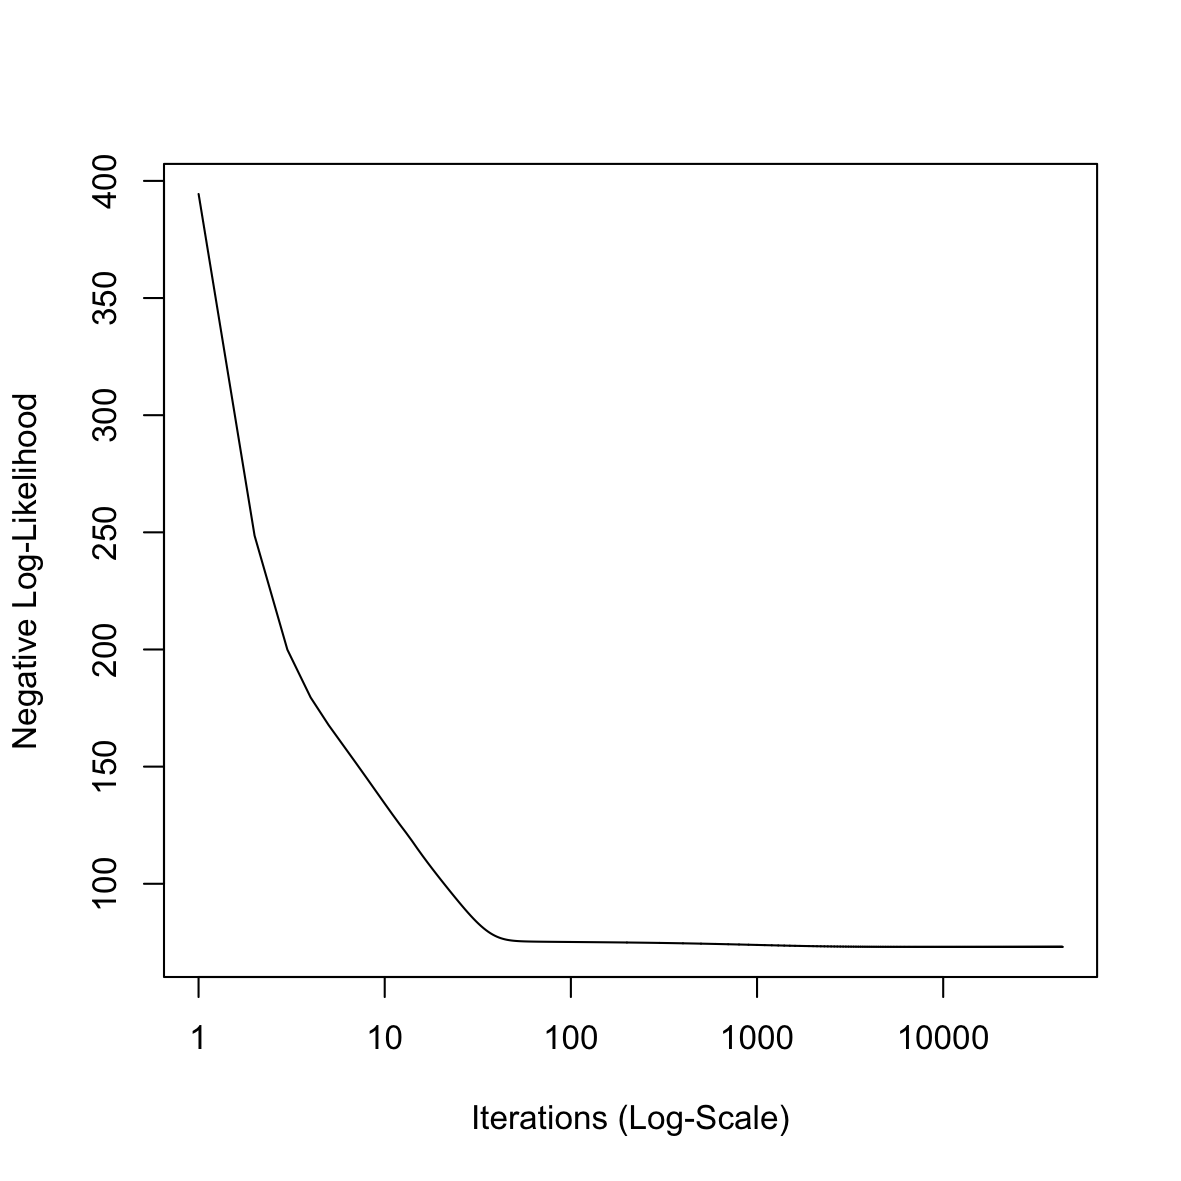
\includegraphics[width=.5\linewidth]{Ex01R/Fig/P2B1.png}
			\caption{Negative log-likelihood optimization using Gradient Descent}
	\end{center}
\end{figure}

The results obtained for the $\hat\beta$ are compared with the results predicted by R function $GLM$:

\begin{table}[ht]
	\small 
	\centering
	\caption{Results for $\hat\beta$ using Gradient Descent and $GLM$ function}
	\label{my-label}
	\begin{tabular}{@{}llllllllllll@{}}
		\toprule
		  & Int. & $\beta_1$ & $\beta_2$  & $\beta_3$  & $\beta_4$  & $\beta_5$  & $\beta_6$  & $\beta_7$  & $\beta_8$  & $\beta_9$  & $\beta_{10}$ \\ \midrule
		Grad Des & 	0.4847 & -7.0987 & 1.6549 & -1.8514 & 13.9863 & 1.0738 & -0.07058 & 0.6761 & 2.5945 &0.4461 & -0.4829    \\
		$GLM$  & 0.4696 & -7.2203 & 1.6499 & -1.7368 & 14.0050 & 1.0736 & -0.07657 & 0.6715 & 2.5804 & 0.4447 & -0.4807  \\ \bottomrule
	\end{tabular}
\end{table}




\newpage
\item Now consider a point $\beta_0 \in \mathcal{R}^P$, which serves as an intermediate guess for our vector of regression coefficients.  Show that the second-order Taylor approximation of $l(\beta)$, around the point $\beta_0$, takes the form
$$
q(\beta; \beta_0) = \frac{1}{2}(z - X \beta)^T W (z - X \beta) + c\, ,
$$
where $z$ is a vector of ``working responses'' and $W$ is a diagonal matrix of ``working weights,'' and $c$ is a constant that doesn't involve $\beta$.  Give explicit expressions for the diagonal elements $W_{ii}$ and for $z_i$ (which will necessarily involve the point $\beta_0$, around which you're doing the expansion).\footnote{Remember the trick of completing the square, e.g.~\url{https://justindomke.wordpress.com/completing-the-square-in-n-dimensions/}.}

\vspace{2mm}
\textbf{Solution}

The second order approximation, as explained by Nocedal and Wright (Equation 2.14), is:

$$ f(x_k + p) \approx f_k + p^T\nabla f_k+\frac{1}{2} p^T\nabla^2f_kp $$

We need to find the second order approximation of $l(\beta)$, around $\beta_0$, and probe that $l(\beta) \approx q(\beta; \beta_0) $. Thus, $x_k = \beta_0$ and $p = \beta-\beta_0$, so we have:

$$ l(\beta) \approx l(\beta_0) + (\beta-\beta_0) ^T\nabla l(\beta_0)+ \frac{1}{2} (\beta-\beta_0)^T \nabla^2 l(\beta_0) (\beta-\beta_0) $$

From Part (A) we know that:
 $$  \nabla l(\beta) =  \displaystyle\sum_{i=1}^{N}\left \{ (m_iw_i - y_i)x_i \right \}=X^T(mw-y)$$  

Now we estimate $\nabla^2 l(\beta_0)$, which is the Hessian:
$$\nabla^2 l(\beta) = \nabla (\nabla l(\beta))  = \nabla \bigg(\displaystyle\sum_{i=1}^{N}\left \{ (m_iw_i - y_i)x_i^T \right \}\bigg) $$

$$\nabla^2 l(\beta) = \displaystyle\sum_{i=1}^{N}\left \{ \nabla_\beta (m_iw_i - y_i)x_i^T \right \} 
=  \displaystyle\sum_{i=1}^{N}\left \{  m_i \nabla _\beta (w_i )x_i^T - 0 \right \} $$

From (A) we have that  $ (\nabla_\beta(w_i))_j=w_i(1-w_i)x_i$ so we can say that, 

$$\nabla^2 l(\beta) =  \displaystyle\sum_{i=1}^{N} m_i w_i(1-w_i)x_i x_i^T = X^TWX$$

Where, $W = m_i w_i(1-w_i)$ is the diagonal matrix of weights. Now we can rewrite the second order approximation of $l(\beta)$,

$$ l(\beta) \approx l(\beta_0) + (mw-y)^TX (\beta-\beta_0)+ \frac{1}{2} (\beta-\beta_0)^T X^TWX (\beta-\beta_0) $$
\newpage
We check on the trick of completing the square from a quadratic form:

$$ a + b^Tx + \frac{1}{2} x^T Cx = \frac{1}{2}(x+m)^T C (x+m) + v $$

We assume that C is symmetric, then: 
$$ m = C^{-1}b $$
$$ v = a - \frac{1}{2}b^TC^{-1}b $$

Now, we apply this trick to the second order approximation of $l(\beta)$ where,
$$ a =  l(\beta_0) $$
$$ b= mw-y $$
$$ x = X \beta - X \beta_0 $$
$$ C = W $$
Then we can find that for our $l(\beta)$:
$$ m = W^{-1} (mw-y) $$
$$ v = l(\beta_0) - \frac{1}{2}(mw-y)^TW^{-1} (mw-y)$$
So we have that:
$$ l(\beta) \approx \frac{1}{2}(x+m)^T C (x+m) + v $$
$$ l(\beta) \approx \frac{1}{2}((X \beta - X \beta_0)+W^{-1} (mw-y))^T W ((X \beta - X \beta_0)+W^{-1} (mw-y)) + l(\beta_0) - \frac{1}{2}(mw-y)^TW^{-1} (mw-y )$$

And we can compared with the equation form we want to show:
$$ q(\beta; \beta_0) = \frac{1}{2}(z - X \beta)^T W (z - X \beta) + c $$

We can observe that c is our $ v = l(\beta_0) - \frac{1}{2}(mw-y)^TW^{-1} (mw-y)$ which is a constant that doesn't involve $\beta$ . And,

$$ z - X \beta = x+m = X \beta - X \beta_0 +  W^{-1} (mw-y) =  X \beta_0 +  W^{-1} (y - mw) - X \beta  $$
$$  z  = X \beta_0 +  W^{-1} (y - mw) $$

Therefore, we showed that $l(\beta) \approx q(\beta; \beta_0) $. Where, $W = m_i w_i(1-w_i)$ and $  z  = X \beta_0 +  W^{-1} (y - mw) $.
\newpage
\item Read up on Newton's method in Nocedal and Wright, Chapter 2.  Implement it for the logit model and test it out on the same data set you just used to test out gradient descent.\footnote{You should be able to use your own solver for linear systems from the first section.}  Note: while you could do line search, there is a ``natural'' step size of 1 in Newton's method.

\vspace{2mm}
\textbf{Solution}

Newton method updates the $\beta$ values in every iteration:

$$ \hat\beta_{i} = \hat\beta_{i-1} - (\nabla^2 l(\hat\beta))^{-1} \nabla l(\hat\beta) $$

The initial guess of beta used is a matrix of zeros with size Px1. The convergence criteria used is the same applied to Gradient Descent function:

$$ \frac{|l(\hat\beta_i) - l(\hat\beta_{i-1})|}{|\hat\beta_{i-1} + \epsilon|} < \epsilon$$

The functions\footnote{The solution is presented in the file $P2B1Function.R$} are developed as follow, 

\begin{lstlisting}[language=R]

# Function 5. Estimate the Hessian of the negative log likelihood
Hessll <- function(b, y, X, m){
# Input:
# b regression parameter P x 1
# y vector of response N x 1
# X Matrix of features N x P
# m number of trial for the ith case
# Output:
# Hessian of l(b) P x 1 

w <- as.numeric(wi.estimate(b, X))
W <- m * w * (1 - w) # Diagonal Matrix of weights
hess <- t(X) %*% diag(W) %*% X
return(hess)
}


# Function 6. Newton Method
NewtonM <- function(y, X, beta, m, iter, epsilon){
# Input:
# iter is the maximum iterations allowed if it doesn't converge
# epsilon is the minimum error allowed for convergency creteria
# Output:
# Negative log likelihood per iteration
# b regression parameter P x 1

# Initial Iteration (GUESS)
betas = array(NA, dim=c(iter, ncol(X)))
betas[1,] = beta
ll = array(NA, dim = iter)
ll[1] = Negll(betas[1,], y, X, m)

# Iterations
for (i in 2:iter){

hess <- Hessll(betas[i-1,], y, X, m) 
grad <- Gradll(betas[i-1,], y, X, m) 

# Improvement direction = Hessian^-1*gradient
dir <- qr.solve(hess, grad) # Using QR decomposition

# Newton Method b=b-Hessian^-1*gradient
betas[i,] <- betas[i-1,] -  dir
ll[i] <- Negll(betas[i,], y, X, m)

# Checking for Convergence
error = abs((ll[i] - ll[i-1])/(ll[i-1] + epsilon))
if (error < epsilon){
cat('Newton Method has converged in iterations:',i)
ll <- ll[1:i]
betas <- betas[1:i,]
break;
}
else if (i == iter & error >= epsilon){
print('Newton Method has not converged')
break;
}
} # for loop
return(list("Negll" = ll, "beta" = betas[i,])) 
}

\end{lstlisting}

\newpage
\textbf{Results}

Based on the code, the function converged in only 10 iterations!!! The values of the negative log-likelihood function for each iteration are presented in the following plot.


\begin{figure}[H]
	\begin{center}
		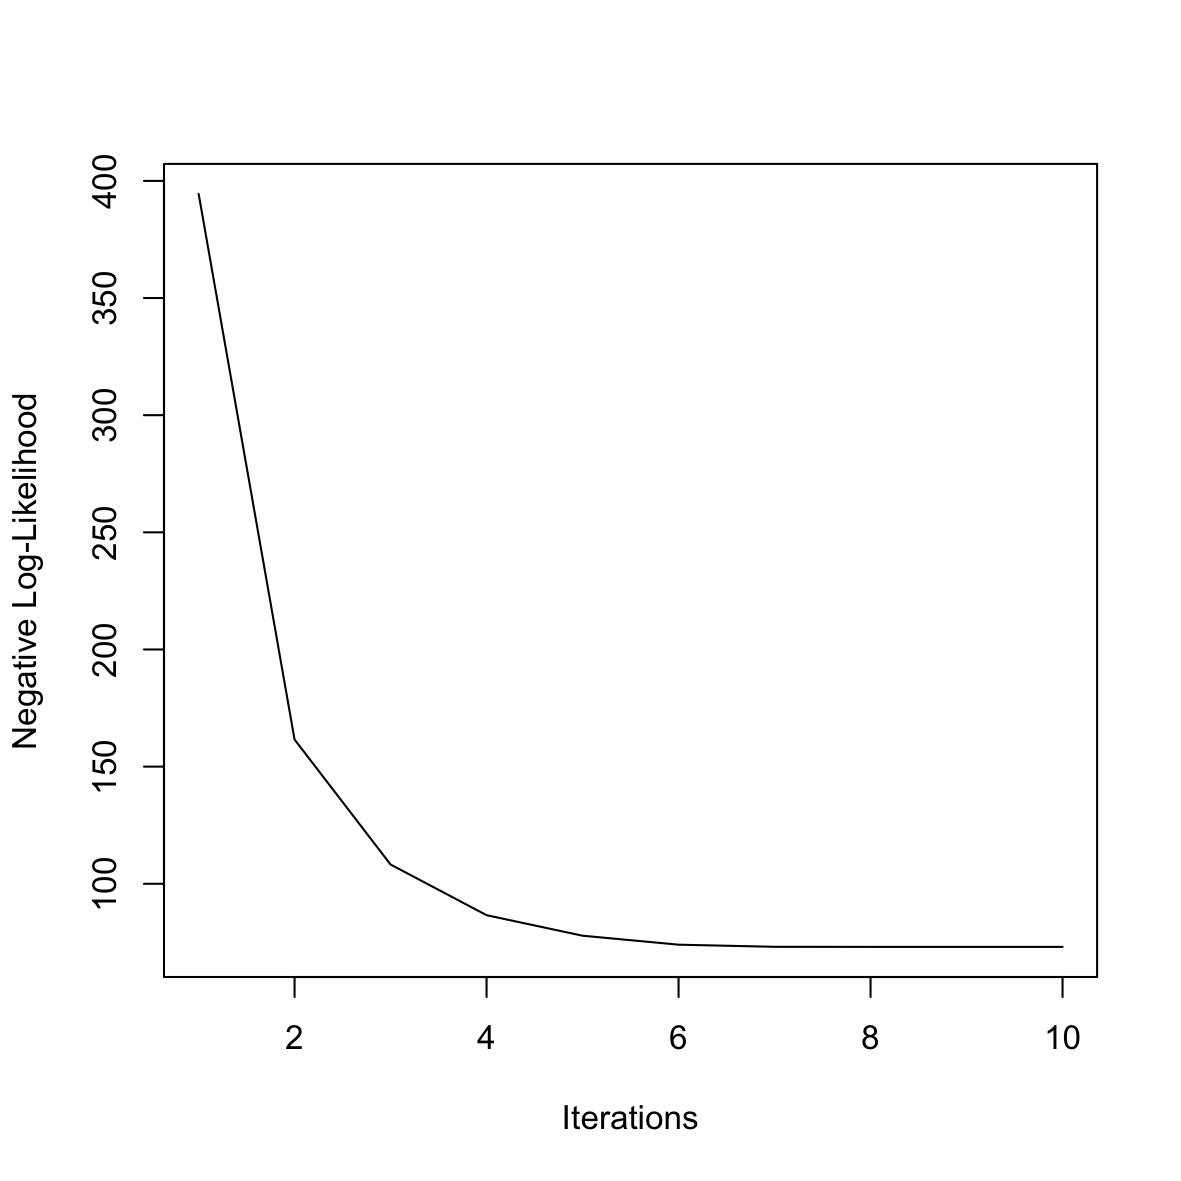
\includegraphics[width=.5\linewidth]{Ex01R/Fig/P2B2.png}
		\caption{Negative log-likelihood optimization using Newton Method}
	\end{center}
\end{figure}

The results obtained for the $\hat\beta$ are compared with the results predicted by R function $GLM$:

\begin{table}[H]
	\small 
	\centering
	\caption{Results for $\hat\beta$ using Newton Method and $GLM$ function}
	\label{my-label}
	\begin{tabular}{@{}llllllllllll@{}}
		\toprule
		& Int. & $\beta_1$ & $\beta_2$  & $\beta_3$  & $\beta_4$  & $\beta_5$  & $\beta_6$  & $\beta_7$  & $\beta_8$  & $\beta_9$  & $\beta_{10}$ \\ \midrule
		Newton & 	0.4847 & -7.2231 & 1.6548 & -1.7372 & 14.0059 & 1.0750 & -0.07723 & 0.6751 & 2.5929 &0.4463 & -0.4825    \\
		$GLM$  & 0.4696 & -7.2203 & 1.6499 & -1.7368 & 14.0050 & 1.0736 & -0.07657 & 0.6715 & 2.5804 & 0.4447 & -0.4807  \\ \bottomrule
	\end{tabular}
\end{table}



\newpage
\item Reflect broadly on the tradeoffs inherent in the decision of whether to use gradient descent or Newton's method for solving a logistic-regression problem.

\vspace{2mm}
\textbf{Solution}

We observe how the Newton Method converged significantly faster than the Gradient Descent. 

The Gradient Descent method has the disadvantage that the value of $\alpha$ to reach converge is not fixed. We need to try various $\alpha$ values. In addition, it can not be big because it oscillates (and it can never converge), and it can not be small cause it takes long time to converge. 

The Newton Method has the disadvantage that we need to estimate the Hessian matrix and also invert it. Invert matrices can be problematic (as studied in the first part of the exercise). We always want to avoid inverting matrices.




\end{enumerate}

\newpage
\bibliographystyle{ieeetr}
\bibliography{references}

\end{document}